\documentclass[aps,pra,preprint,superscriptaddress,floatfix]{revtex4-2}
\usepackage{amsmath,amssymb}
\usepackage{graphicx}
\graphicspath{{figures/}}

\begin{document}
\title{Supplemental Material for ``Short-pulse sequences as local probes for
superconducting-qubit frequency calibration''}
\author{Zhouyi Rao}
\affiliation{Institute of Physics, Chinese Academy of Sciences, Beijing 100190, China}
\affiliation{University of Chinese Academy of Sciences, Beijing 100049, China}
\maketitle

\section{Frequency--flux response}

Figure~\ref{fig:flux-curve} compares analytic, Ramsey, and transient estimates
over a wider flux interval.  The fixed-drive transient error grows sharply at
the edge because the resulting detuning leaves the local response window.

\begin{figure}[t]
 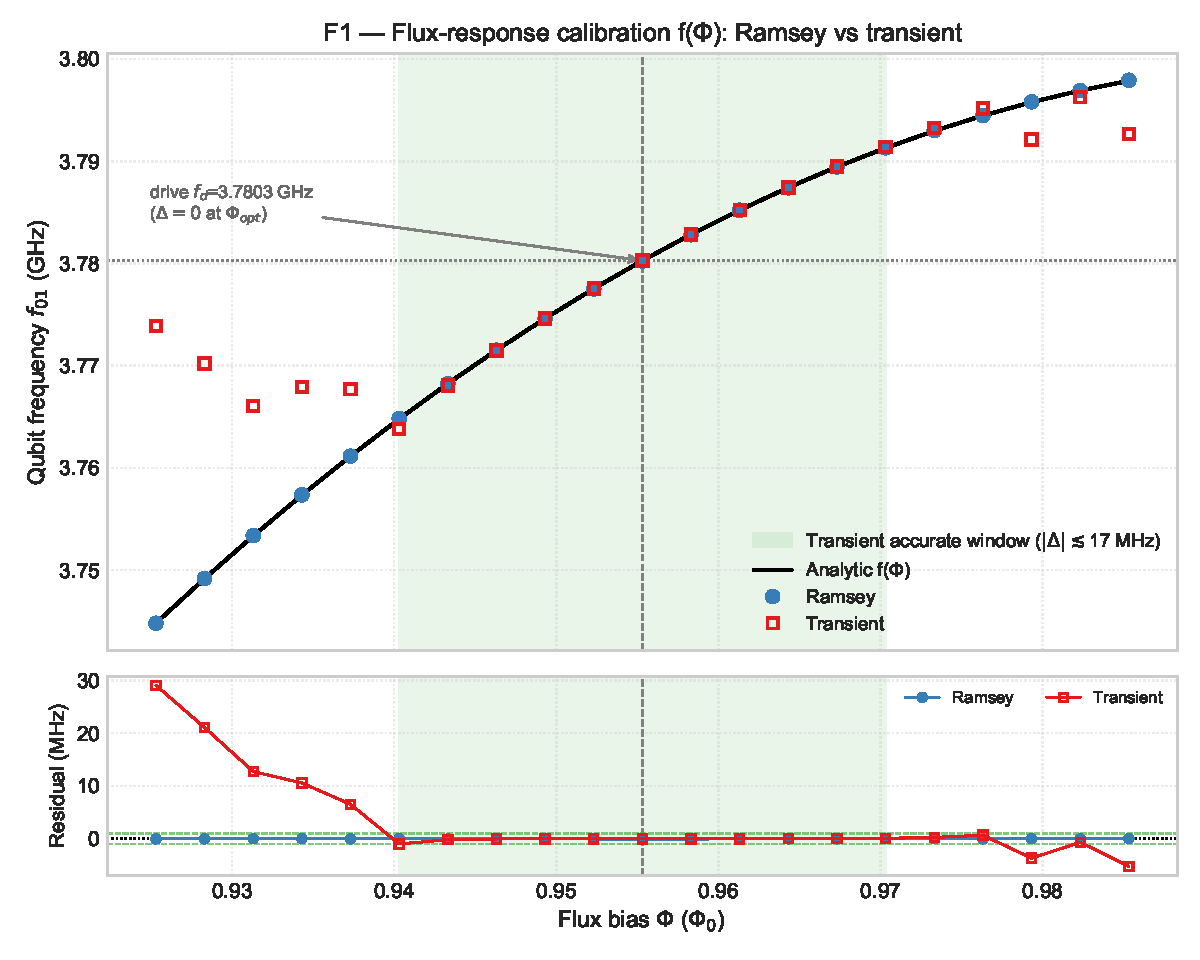
\includegraphics[width=\textwidth]{flux_curve.pdf}
 \caption{Frequency--flux response and residuals over an extended interval.}
 \label{fig:flux-curve}
\end{figure}

\section{Root-finding updates}

Figure~\ref{fig:step-methods} compares secant, bisection, and damped-gradient
updates using the same Ramsey frequency measurement.  This separates the
choice of controller update from the transient measurement studied in the main
text.

\begin{figure}[t]
 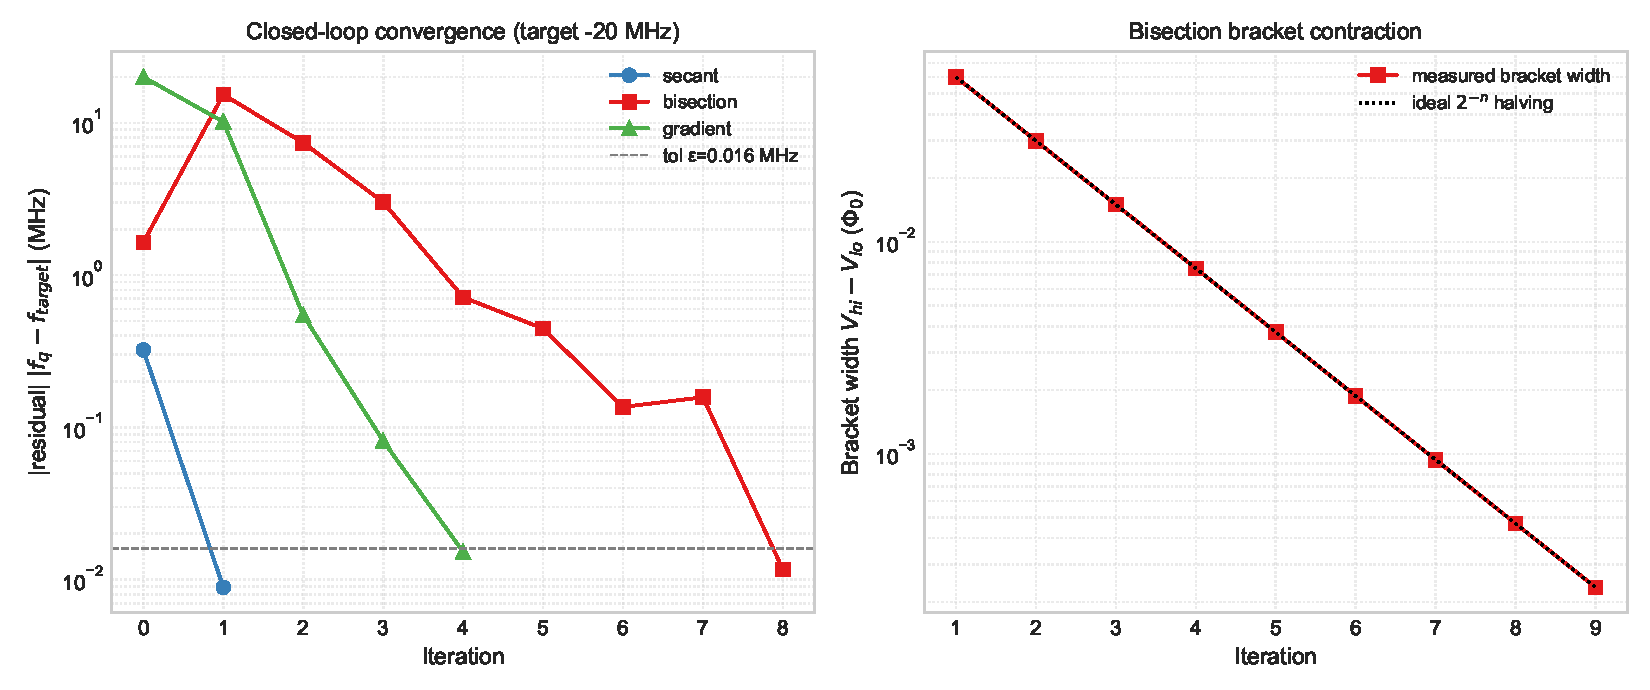
\includegraphics[width=\textwidth]{step_methods.pdf}
 \caption{Closed-loop convergence for three root-finding updates and the
 bisection bracket width.}
 \label{fig:step-methods}
\end{figure}

\section{Experimental extensions}

An experimental implementation should add binomial shot sampling, readout
assignment correction, repeated calibrations under controlled drift, and a
range-guard transition to Ramsey reacquisition.  Coefficients $A_1$ and $A_3$
should be remeasured after material pulse-shape or drive-chain changes.

\end{document}
